\documentclass[border=8pt]{standalone}
\usepackage{pgfplots}
\pgfplotsset{compat=1.18}
\begin{document}
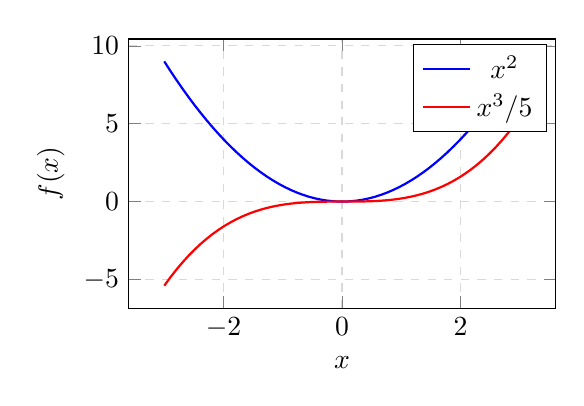
\begin{tikzpicture}
  \begin{axis}[
    xlabel={$x$},
    ylabel={$f(x)$},
    width=7cm, height=5cm,
    grid=major,
    grid style={dashed, gray!30}
  ]
    \addplot[blue, thick, domain=-3:3, samples=60]{x^2};
    \addlegendentry{$x^2$}
    \addplot[red, thick, domain=-3:3, samples=60]{x^3/5};
    \addlegendentry{$x^3/5$}
  \end{axis}
\end{tikzpicture}
\end{document}
